\documentclass[dvipsnames,pdflatex,beamer]{beamer}
%\documentclass[dvipsnames,pdflatex,handout]{beamer}
%                                   ^^^^^^^ << for handout - happens in Makefile
\usepackage[english]{babel}
\usepackage[utf8]{inputenc}
%beamer breaks with\usepackage{paralist}%-> {compactenum}, ... (Aargh!)
%\usepackage{mdwlist}% \suspend and \resume enumerate
\usepackage{relsize}% ``relative font sizes''
%% part of {mmVignette} below: \usepackage{SweaveSlides}
\usepackage{mmVignette}%-- local in this directory: -> {listings}, \lstset,...
%           ^^^^^^^^^^
\usepackage{MM-slides}% whitespace-tricks, \nlQ etc
\usepackage{MM-colors}% {\color{salmonII} ..text..} \textcolor{red}{..txt..}
%\usepackage{bm}
%-------------------------------------------------------------
%
\newcounter{saveenum}
\newcommand*{\Rp}{\textsf{R}$\;$}% R program
\newcommand*{\CRAN}{\textsc{cran}$\;$}
\newcommand*{\W}{\ensuremath{\mathbf{W}}}
\newcommand*{\Ip}{\mathbf{I}_p}
%---- from texab.sty --- can not take all --------------
% \newcommand{\norm}[1]   {\left\| #1 \right\|}
% % the above sometimes give much too long  || -- then use the following:
% \newcommand{\normb}[1]  {\bigl\|{#1}\bigr\|}
% \newcommand{\normB}[1]  {\Bigl\|{#1}\Bigr\|}
\newcommand{\fn}[1]{\kern-2pt\left(#1\right)}
\newcommand{\Ew}[1]{\mathbf{E}\kern2pt\fn{#1}}
%
%
\mode<handout>{\usetheme{default}}
\mode<beamer>{%
  %%> http://www.namsu.de/latex/themes/uebersicht_beamer.html
  \usetheme{Boadilla}% somewhat similar to Singapore, but "nice" blocks
  %\usetheme{Singapore}%  \usetheme{Madrid}%
  \setbeamercovered{dynamic}% {transparent} {invisible} or {dynamic}
  % Use ETH Logo
%   \pgfdeclareimage[height=0.5cm]{ETH-logo}{../ethlogo_black}%
%   \logo{\pgfuseimage{ETH-logo}}%
  % \pgfdeclareimage[height=0.5cm]{R-logo}{Rlogo}%
  \pgfdeclareimage[height=0.5cm]{R-logo}{useR}%
  \logo{\pgfuseimage{R-logo}}%
}
\usefonttheme[onlymath]{serif}



\title[Sparse Matrices in \texttt{Matrix} pkg]{%
Sparse Matrices in package Matrix and applications
}

\author[Martin Maechler, Doug Bates]{Martin Maechler and Douglas Bates}
\institute[R Core]{% 'ETH Z' if more needed
  Seminar für Statistik \\ ETH Zurich  \ \ Switzerland

  \bigskip

  Department of Statistics \\ University of Madison, Wisconsin \ \ U.S.A.

  {\color{Scode}\texttt{(maechler|bates)@R-project.org} \ \ (R-Core)}
}
\date[useR!, Rennes 2009]{useR! 2009, Rennes \\ July 10, 2009}

\begin{document}

\begin{frame} \titlepage
\end{frame}
%
\begin{frame} \frametitle{Outline}
  \tableofcontents
  % You might wish to add the option [pausesections]
\end{frame}

\section[Intro]{Introduction to Matrix and Sparse Matrices}\label{sec:intro}
\begin{frame}\frametitle{Introduction}
  \begin{itemize}
  \item<1-2> \texttt{Matrix}: \pause the movie
  \item<3-> \texttt{Matrix}: the R package :

    \bigskip

  \item<4-> Package \texttt{Matrix}: a \alert{recommended} R package since R 2.9.0
  \item<4-> Infrastructure for other packages for several years,
    notably \pkg{lme4}\footnote{
      \alert{lme4} := (Generalized--) (Non--) \alert{L}inear \alert{M}ixed
      \alert{E}ffect Modelling,
      \\ \qquad\qquad
      (using S\alert{4} $\mid$ re-implemented from scratch the
       $\alert{4}^\mathrm{th}$ time)}

  \item<4-> CRAN nowadays lists direct ``reverse dependencies'':
  \end{itemize}
\end{frame}

\begin{frame}\frametitle{(reverse) Dependencies on Matrix}
  On June 26, 2008 ($>$ one year ago), Matrix was not yet recommended,
  and had the following CRAN dependency graph:
\hspace*{-6mm}
  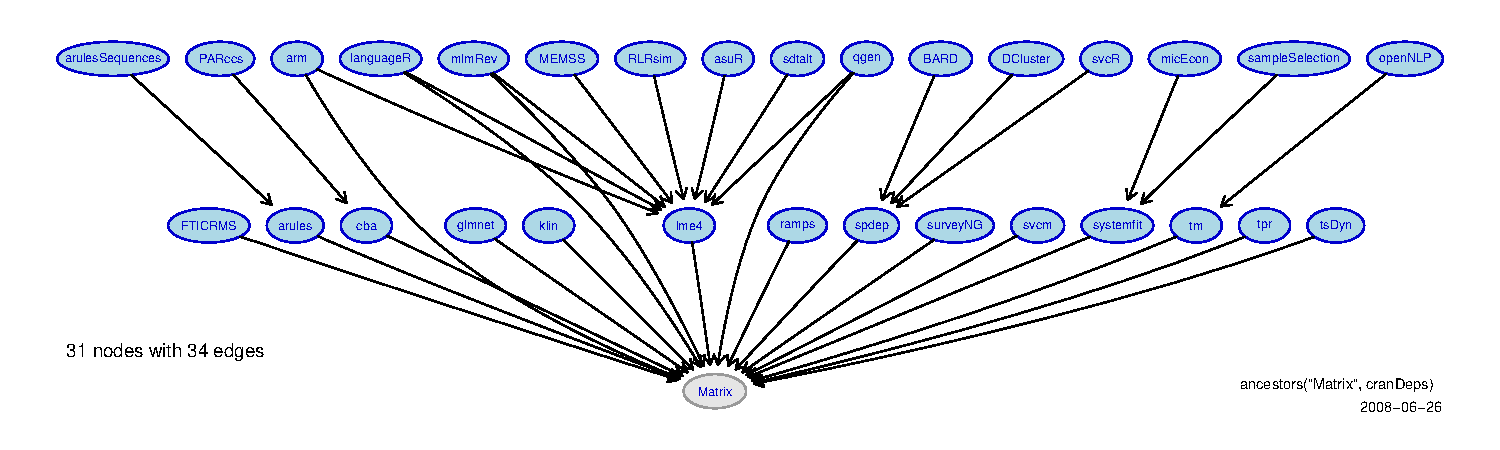
\includegraphics[width=1.1\textwidth]{figs/deps-on-Matrix2008-06}

  i.e., 14 + 1 directly dependent packages.
\end{frame}

\begin{frame}\frametitle{Dependencies on Matrix -- 2009-07}
  Today, quite a few more packages depend on Matrix explicitly:

  CRAN $\to$ Packages $\to$ Matrix  \ \ \     displays the following \\
   \qquad\qquad \url{http://cran.r-project.org/web/packages/Matrix/}

   \begin{block}{}
     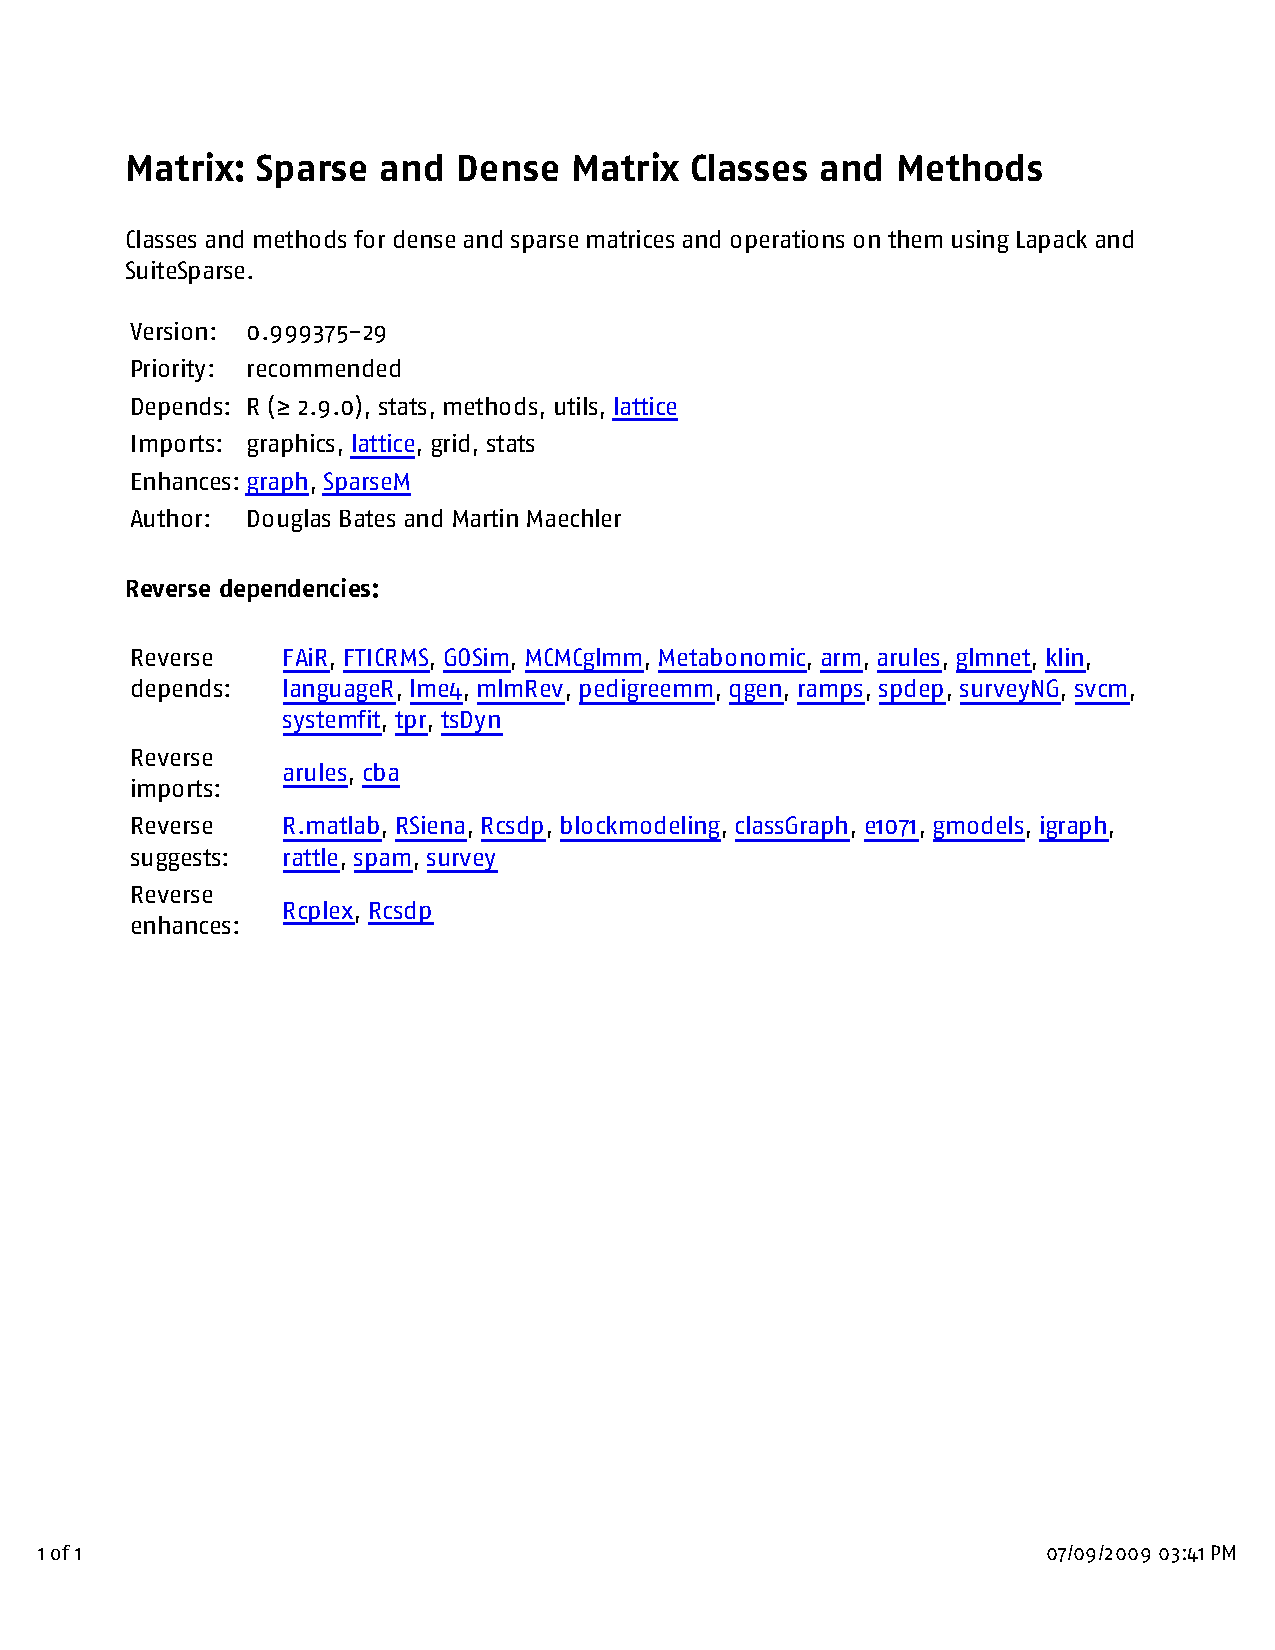
\includegraphics[width=1.\textwidth,viewport=40 400 580 730,clip]{figs/Matrix-CRAN-depend-2}
   \end{block}
\end{frame}

\begin{frame}
 \url{http://cran.r-project.org/web/packages/Matrix/} :

 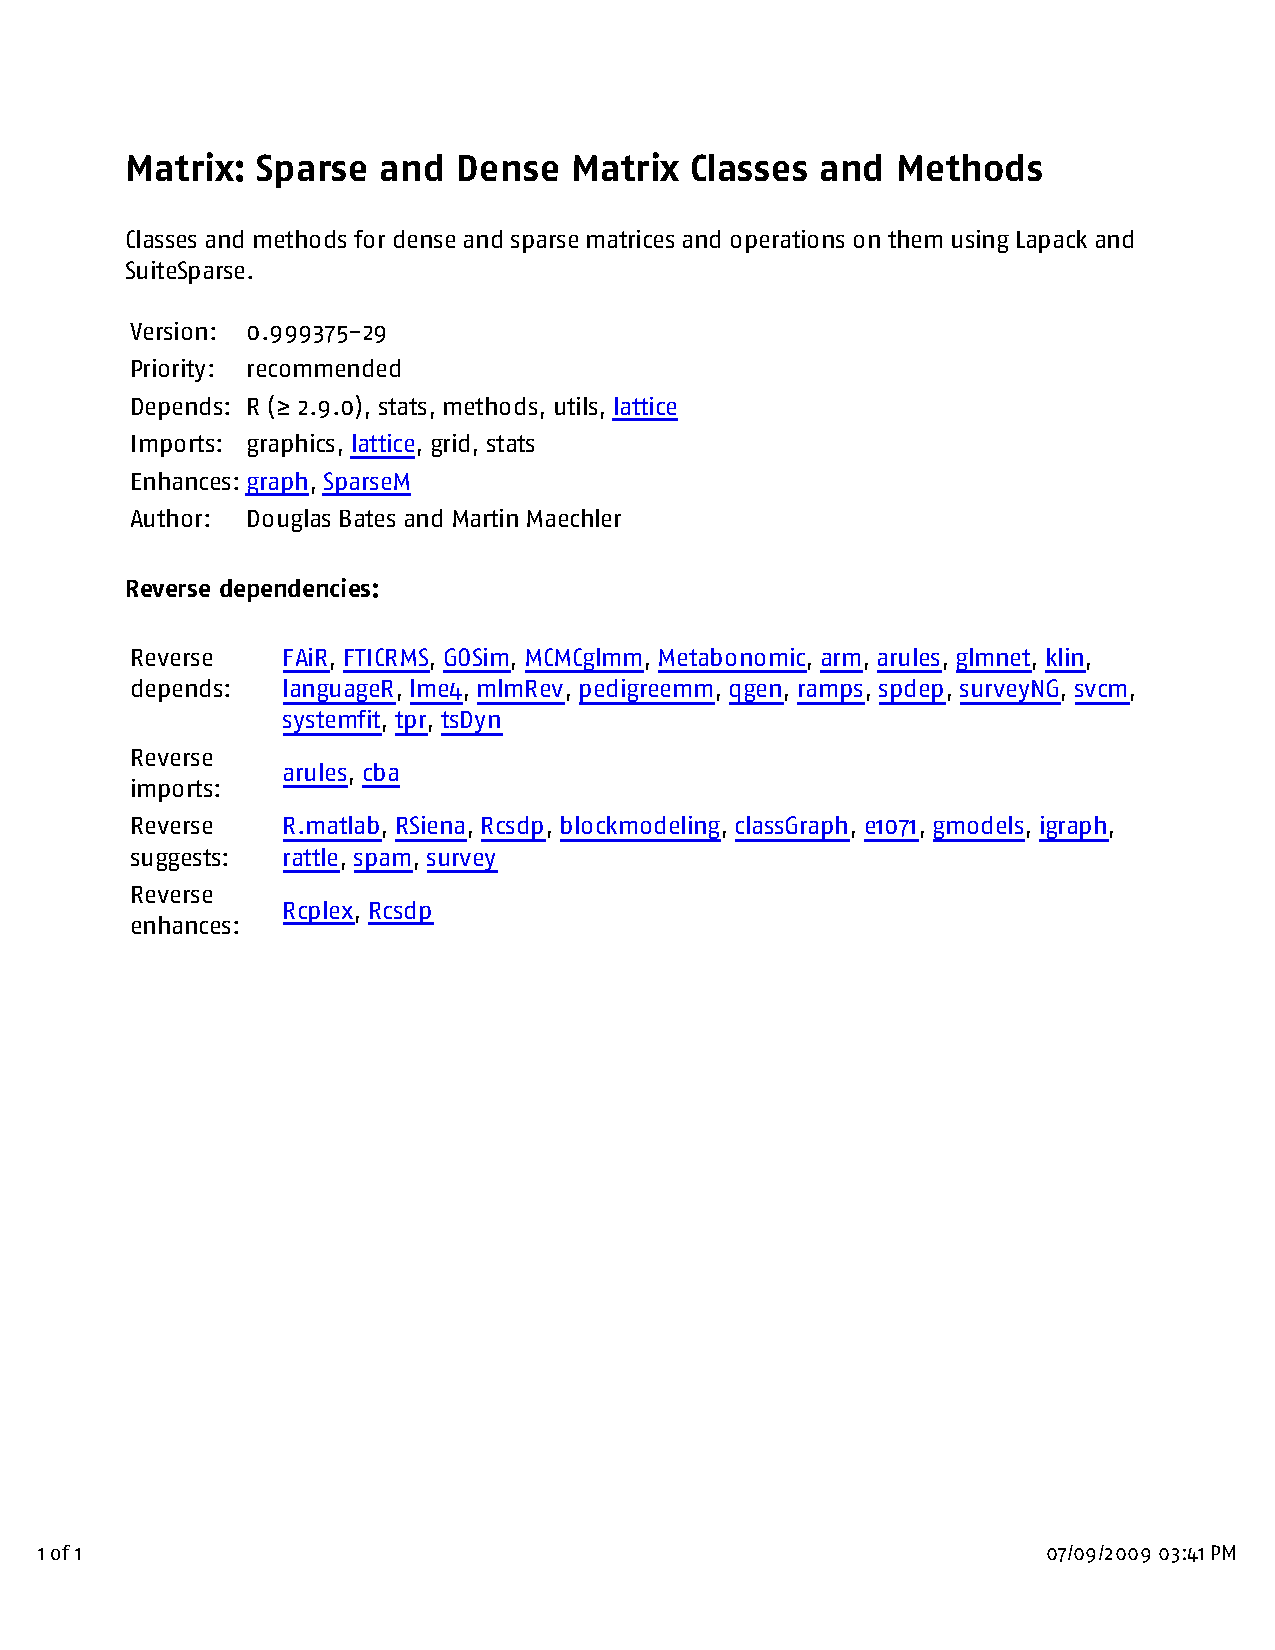
\includegraphics[width=1.\textwidth,viewport=40 0 580 730,clip]{figs/Matrix-CRAN-depend-2}

\end{frame}

\begin{frame}\frametitle{Dependencies on Matrix --- 2009-07 --- Summary}

  \begin{enumerate}
  \item After one year, we have 22 (up from 15) packages depending on Matrix
    explicitly, plus another 12  ``suggest'' or ``enhance'' it.

  \item Notably \pkg{glmnet}, Trevor Hastie's favorite in yesterday's keynote.

  \item Most important one: \pause \alert{lme4} and \emph{its} dependencies
  \end{enumerate}

%   \fbox{34} CRAN packages now depend (\fbox{22}) or suggest/enhance (12)
%   ``Matrix''.
\end{frame}

\input{sparse-intro-09}

\input{Matrix-classes-123}

%%--------------
\input{SAR1}%-> SAR1.Rnw
%%--------------

\section{Application - Mixed Modelling (RE)ML in R}\label{sec:lmer}
\begin{frame}\frametitle{Mixed Modelling - (RE)ML Estimation in pure R}
In (linear) mixed effects, the evaluation of the (RE)
likelihood or equivalently deviance, needs repeated Cholesky decompositions
of
\begin{equation}
  \label{eq:U'U+I}
  \bU_\theta \bU_\theta\tr + \bI,
\end{equation}
for many $\theta$ values ($=$ the relative variance components)
and (often very large), very sparse matrix
$\bU_\theta$ where only the \emph{non}-zeros of $\bU$ depend on $\theta$,
i.e., the sparsity pattern is given (by the observational design).

Sophisticated (fill-reducing) Cholesky done in two phases:
\begin{enumerate}
\item ``symbolic'' decomposition: Determine the non-zero entries of $\bm L$
  ($\bm L {\bm L}\tr = \bU \bU\tr + \bI$),
\item numeric phase: compute these entries.

Phase 1: typically takes much longer; only needs to happen \emph{once}.\\
Phase 2: ``update the Cholesky Factorization''
\end{enumerate}
\end{frame}

%%--------------
\input{ETH-teachers}%-> ./ETH-teachers.Rnw
%%--------------

\begin{frame}\frametitle{Summary}

\begin{itemize}[<+->]
 \item Recommended \RR\ package "Matrix"
 \item \emph{Sparse} Matrices: in increasing number of applications
 \item S4 classes and methods are \alert{the} natural implementation tools

 \item lme4 is going to contain an alternative ``pure R'' version of ML and REML,
   you can pass to \texttt{nlminb()} \textcolor{gray}{(or \texttt{optim()}
     if you must :-)}.
   UseRs can easily extend these R functions to more flexible models or
   algorithms.

 \item Matrix 1.0-0
   \begin{enumerate}[<+->]
   \item will happen
   \item will contain \texttt{sparse.model.matrix()}
   \item will contain truly sparse \texttt{lm(*, sparse=TRUE)}
   \end{enumerate}
\end{itemize}
\pause

\bigskip

\bigskip
\begin{block}{}
   That's all folks --- with thanks for your attention!
\end{block}

\end{frame}

\end{document}

%%% Local Variables:
%%% mode: latex
%%% TeX-command-default: "LaTeX PDF"
%%% TeX-master: t
%%% End:
